\chapter{ทฤษฎีความรู้และงานที่เกี่ยวข้อง}

\emph{หัวข้อต่าง ๆ ในแต่ละบทเป็นเพียงตัวอย่างเท่านั้น หัวข้อที่จะใส่ในแต่ละบทขึ้นอยู่กับโปรเจคของนักศึกษาและอาจารย์ที่ปรึกษา}

ตัวอย่างการใส่อ้างอิงที่มา -> \cite{hypersense} ถ้าต้องการใส่แหล่งอ้างอิงมากกว่า 1 ให้ทำดังนี้ -> \cite{hypersense,bworld}
อธิบายทฤษฎี องค์ความรู้หลักที่ใช้ในงาน งานวิจัยที่นำมาใช้ในโครงงาน หรือเปรียบเทียบผลิตภัณฑ์ที่มีอยู่ในท้องตลาด\cite{bworld}
Explain theory, algorithms, protocols, or existing research works and tools related to your work.


% \section{ระบบแนะนำสินค้า}

% \begin{table}[!h]
%     \caption{test table method1}\label{tbl:method1}
%     \begin{tabular}{c|c|l|rr} \hline\hline
%         Center & Center & left aligned & Right & Right aligned \\ \hline\hline
%         Center & Center & left aligned & Right & Right aligned \\ \hline
%         Center & Center & left aligned & Right & Right aligned \\
%         Center & Center & left aligned & Right & Right aligned \\ \hline
%         Center & Center & left aligned & Right & Right aligned \\ \hline\hline
%     \end{tabular}
% \end{table}

\section{อัลกอริทึมในการแปลผลภาษา}
\subsection{Term Frequency Inverse Document Frequency (TF-IDF)}
เป็นอัลกอริทึมที่ผสมผสานกันระหว่าง Term-Frequency (TF) และ Inverse Document Frequency (IDF) ซึ่งเป็น
เทคนิคพื้นฐานเทคนิคหนึ่งที่ใช้ในการวิเคราะห์ค้นหาคำสำคัญของข้อมูลในลักษณะของข้อความ
\begin{itemize}
    \item \textbf{Term-Frequency (TF)} โดยจะคำนวณเป็นอัตราส่วนของจำนวนคำนั้น ๆ ต่อจำนวนคำทั้งหมดในเอกสาร
    เพื่อหาว่าคำนั้นมีความถี่เท่าไหร่
    \begin{figure}[!h]\centering
        \setlength{\fboxrule}{0.2mm} % can define this in the preamble
        \setlength{\fboxsep}{1cm}
        \fbox{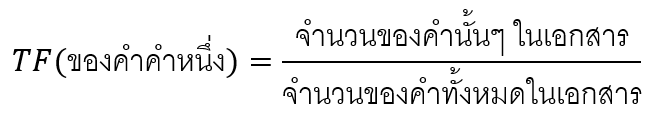
\includegraphics[width=5cm]{./figure/figure_tf.png}}
        \caption{สมการการคำนวณ Term-Frequency (TF)}\label{fig:model4}
    \end{figure}
    \item \textbf{Inverse Document Frequency (IDF)} โดยจะคำนวณความสำคัญของแต่ละคำโดยคำที่พบได้บ่อยจะมีค่า IDF ที่ต่ำ
    ซึ่งบ่งบอกว่าคำเหล่านั้นไม่สามารถดึงเอาจุดเด่นของเอกสารออกมาได้ดี
    \begin{figure}[!h]\centering
        \setlength{\fboxrule}{0.2mm} % can define this in the preamble
        \setlength{\fboxsep}{1cm}
        \fbox{
\includegraphics[width=5cm]{./figure/figure_idf.png}}
        \caption{สมการการคำนวณ Inverse Document Frequency (IDF)}\label{fig:model5}
    \end{figure}
    \item \textbf{คำนวณค่า TF-IDF} โดยเราจะนำ TF กับ IDF มาคำนวณและถ้าหากคำไหนที่มาค่า TF-IDF ที่สูง จะถูกมองว่าเป็นคำที่มีความสำคัญ
    สูง (กล่าวถึงบ่อย แต่ก็ไม่ได้ปรากฏอยู่หลายเอกสารเกินไป) และมีแนมโน้มจะเป็นใจความสำคัญของเอกสาร
    \[TFIDF = TF * IDF\]
\end{itemize}


\section{อัลกอริทึมในการแยกประเภทเรซูเม}
\subsection{อัลกอริทึม I K-Nearest Neighbors (KNN)}

% Can define this in the preamble..
เป็นอัลกอริทึมสำหรับการจัดกลุ่มข้อมูล (Classfication) ซึ่งอยู่ในกลุ่มของการเรียนรู้แบบมีผู้สอน (Supervised Learning)
หลักการทำงาน คือการจัดกลุ่มโดยอิงถึงความใกล้เคียงของข้อมูล เพื่อคาดเดาหรือจำแนกประเภทข้อมูลใหม่ โดยหลักการทำงานสามารถสรุปได้ดังนี้
\begin{enumerate}
    \item  \textbf{เลือกค่า K} : กำหนดค่า K ที่ต้องการ ซึ่งเป็นจำนวนของข้อมูลที่ใกล้ที่สุดที่จะใช้ในการตัดสินใจ
    \item  \textbf{คำนวณระยะทาง} : ใช้ระยะทางยูคลิเดียน (Euclidean distance) เพื่อคำนวณหาความคล้ายคลึงระหว่างข้อมูล
    \item  \textbf{หาข้อมูลที่ใกล้ที่สุด} : หลังจากคำนวณระยะทางระหว่างข้อมูลทดสอบกับข้อมูลในชุดข้อมูลการฝึกฝน เราจะเลือกข้อมูล K รายการที่มีระยะทางน้อยที่สุด
    \item  \textbf{คำนวณผลโหวต} : เมื่อเราได้ข้อมูล K รายการที่ใกล้ที่สุดแล้ว เราจะนับจำนวนรายการในแต่ละกลุ่มหรือประเภทข้อมูล 
    และกำหนดกลุ่มหรือประเภทข้อมูลของข้อมูลทดสอบตามจำนวนที่มากที่สุดใน K รายการนั้น
    \item  \textbf{ทำนายผลลัพธ์} : สุดท้ายเราก็จะได้กลุ่มข้อมูลที่ถูกแบ่งออกมาพร้อมใช้ในการทำนายต่อไป
\end{enumerate}

\begin{figure}[!h]\centering
    \setlength{\fboxrule}{0.2mm} % can define this in the preamble
    \setlength{\fboxsep}{1cm}
    \fbox{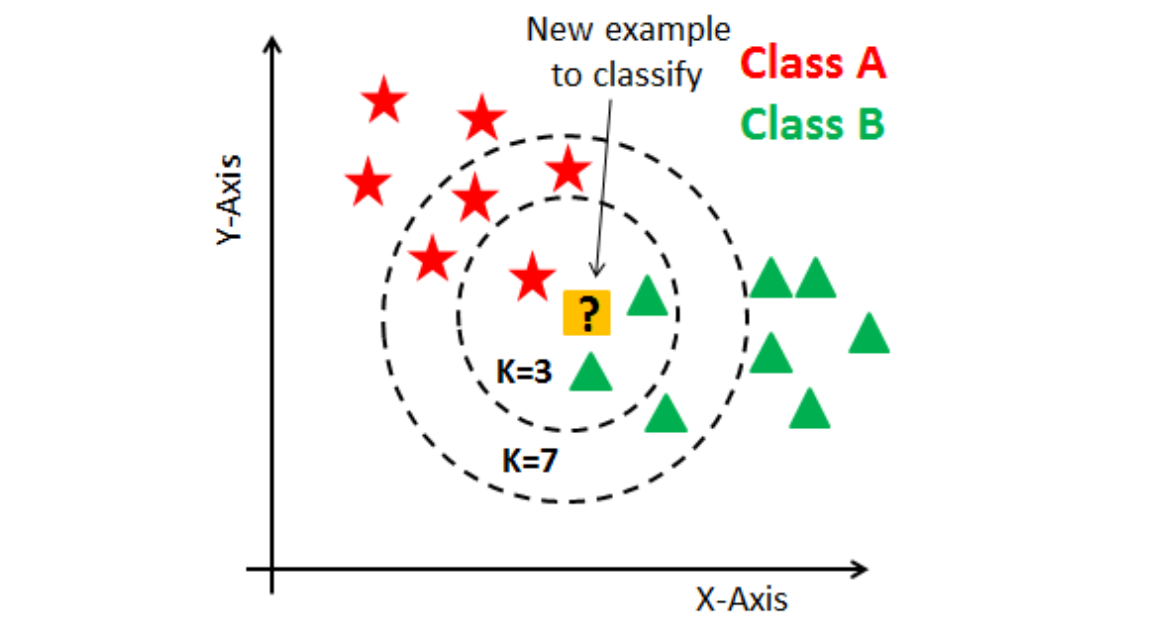
\includegraphics[width=5cm]{./figure/figure_knn.png}}
    \caption{ลักษณะการทำงานของ K-Nearest Neighbors}\label{fig:model2}
\end{figure}

\subsection{อัลกอริทึม II Naive Bayes Classifier}
Naive Bayes Classification เป็นหนึ่งใน Classification Model ใช้ในการแบ่งกลุ่มหรือหาเหตุการณ์ที่จะเกิดขึ้นโดยการอิงทฤษฎีความน่าจะเป็นของ 
Bayes หรือ Bayesian 
\par ซึ่งจะคำนวณว่าจะเกิดเหตุการณ์นั้นหรือไม่โดยจะเพิ่มโอกาสในการเกิดเหตุการณ์เข้าไปด้วย 
โดยมักจะใช้ในการวิเคราะห์ข้อมูลที่มีความต่อเนื่องของเหตุการณ์ (Dependent Event) เช่น 
โอกาสในการเกิดโรคในกลุ่มประชากรที่เราสนใจ ซึ่งจำเป็นจะต้องอาศัยการคำนวณผ่านสูตรดังนี้ และกำหนดให้

\begin{figure}[!h]\centering
    \setlength{\fboxrule}{0.2mm} % can define this in the preamble
    \setlength{\fboxsep}{1cm}
    \fbox{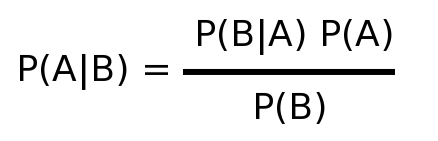
\includegraphics[width=5cm]{./figure/figure_nb.png}}
    \caption{สมการความน่าจะเป็นของ Bayes หรือ Bayesian}\label{fig:model3}
\end{figure}

\par P(A|B) คือความน่าจะเป็นในการเกิดเหตุการณ์ A โดยมี B เป็น Condition
\par P(B|A) คือความน่าจะเป็นในการเกิดเหตุการณ์ B โดยมี A เป็น Condition
\par P(A) คือโอกาสในการเกิดเหตุการณ์ A จากเหตุการณ์ทั้งหมด
\par P(B) คือโอกาสในการเกิดเหตุการณ์ B จากเหตุการณ์ทั้งหมด



\section{การศึกษาข้อมูลผลิตภัณฑ์ที่ใกล้เคียง}
\subsection{หนังสือหลักสูตรวิศวกรรมศาสตร์บัณฑิต สาขาวิศวกรรมคอมพิวเตอร์ มจธ.}
เป็นหนังสือที่บอกถึงรายละเอียดของแต่ละรายวิชาที่นักศึกษาวิศวกรรมคอมพิวเตอร์ได้เรียนในหลักสูตรตั้งแต่ปี 1 ถึงปี 4
โดยจะแสดงออกมาเป็นผลลัพธ์การเรียนรู้และทักษะที่ได้จากการเรียนในวิชาต่าง ๆ แต่จะไม่ได้บอกถึงอาชีพสามารถนำไปต่อยอดจากรายวิชาได้
\par ซึ่งทางคณะผู้จัดจะนำข้อมูลรายวิชาในแต่ละปีการศึกษามาศึกษามาแบ่งว่า แต่ละรายวิชาสามารถนำไปต่อยอดทางใดได้บ้าง 
เพื่อมาวางแผนเส้นทางการลงวิชาเลือกที่สัมพันธ์กับระดับการศึกษาและความสนใจของผู้ใช้งานแต่ละคน

\subsection{LinkedIn}
LinkedIn เป็นเว็บแอปพลิเคชันชุมชนในสายอาชีพต่าง ๆ ที่ช่วยให้ผู้ใช้สร้างโปรไฟล์อาชีพของตนเองและเชื่อมโยงกับคนที่ใกล้เคียงในสายอาชีพ 
เว็บไซต์นี้จะช่วยให้ผู้ใช้สามารถสร้างเครือข่ายในสายอาชีพของตน แบ่งปันข้อมูลเกี่ยวกับประสบการณ์การทำงาน ประวัติการศึกษา ทักษะ ความถนัด 
รวมถึงเผยแพร่เนื้อหาที่เกี่ยวข้องกับสาขาอาชีพของพวกเขาในรูปแบบข่าวสาร ทำให้เชื่อมโยงและแลกเปลี่ยนข้อมูลกับผู้ใช้อื่น ๆ ในวงการได้ตลอดเวลา \\
โดยที่เว็บไซต์มีฟังก์ชันหลายอย่าง ประกอบด้วย :
\begin{itemize}
    \item \textbf{โปรไฟล์ผู้ใช้} : ผู้ใช้สามารถสร้างโปรไฟล์ส่วนตัวที่แสดงประสบการณ์การทำงาน การศึกษา ทักษะ และข้อมูลอื่นๆ เพื่อให้ผู้ใช้อื่นสามารถทราบรายละเอียดเบื้องต้นของพวกเขาได้
    \item \textbf{การเชื่อมโยง} : ผู้ใช้สามารถเชื่อมโยงกับคนอื่นในสายอาชีพ ทำให้สร้างเป็นเครือข่ายในสายอาชีพที่แข็งแกร่งขึ้น และเป็นโอกาสที่ดีให้กับผู้ใช้งานได้
    \item \textbf{โพสต์และเนื้อหา} : ผู้ใช้สามารถโพสต์เนื้อหาเกี่ยวกับวงการอาชีพ เช่น บทความ ข่าวสาร และความคิดเห็น ซึ่งช่วยในการแบ่งปันความรู้และประสบการณ์
    \item \textbf{ค้นหางาน} : ผู้ใช้สามารถค้นหางานและสมัครงานได้โดยตรงผ่านแพลตฟอร์ม และผู้ประกาศงานก็สามารถค้นหาผู้สมัครที่เหมาะสมกับตำแหน่งงานที่ว่างอยู่ของตนเองได้โดยง่าย
    \item \textbf{กลุ่มองค์กร} : บริษัทและองค์กรสามารถสร้างหรือเข้าร่วมกลุ่มบน LinkedIn เพื่อแบ่งปันข้อมูลและความรู้ในหมวดหมู่ที่เกี่ยวข้องได้ภายในกลุ่มที่กำหนดเองได้
    \item \textbf{การแสดงความสนใจ} : ผู้ใช้สามารถกดถูกใจ แสดงความคิดเห็น หรือแชร์เนื้อหาของผู้อื่น เพื่อแสดงความรับรู้ สนใจ หรือช่วยในการประกาศข่าวสารที่ดี
\end{itemize}
\par ซึ่งถือว่าเป็นเว็บแอปพลิเคชันที่เกี่ยวข้องกับการหางานที่มีความสามารถที่สูง และเน้นไปที่การสร้างคอมมูนิตี้สำหรับการทำงาน เนื่องด้วยคุณสมบัติที่หลากหลายนี้ 
ทำให้มีผู้ใช้งานเป็นจำนวนมาก ซึ่งทางคณะผู้จัดทำจะนำระบบชุมชนที่สามารถแนะนำงานกับกิจกรรม และระบบจัดเก็บเรซูเมมาต่อยอดกับโครงงานของเราให้ดียิ่งขึ้น

\subsection{JobDB}
เป็นเว็บแอปพลิเคชันที่รวบรวมตำแหน่งงานต่าง ๆ ในประเทศไทยที่กำลังเปิดรับอยู่ ที่จัดทำขึ้นมาสำหรับผู้คนที่กำลังมองหางาน \\
โดยที่เว็บไซต์มีฟังก์ชันหลายอย่าง ประกอบด้วย :
\begin{itemize}
    \item ระบบค้นหาอาชีพที่ต้องการ
    \item โพสต์ที่จะมีรายละเอียดงานที่เปิดรับ
    \item ระบบสมัครงาน
    \item คำแนะนำสำหรับการจัดทำเอกสารการสมัครงาน
    \item การแจ้งเตือนสำหรับตำแหน่งงานที่ผู้ใช้งานสนใจ
\end{itemize}
\par ซึ่งเป็นเว็บแอปพลิเคชันรวบรวมตำแหน่งงานที่เน้นกลุ่มเป้าหมายเป็นผู้ที่กำลังหางานในประเทศไทย โดยรวมมีระบบที่คอยอำนวยความสะดวกในการค้นหางานที่ผู้ใช้งานสนใจ 
และยังมีฟังก์ชันที่น่าสนใจเป็นอย่างมากกับ ระบบคำแนะนำสำหรับการจัดทำเอกสารการสมัครงาน ซึ่งทางผู้จัดทำโครงงานจะนำฟังก์ชันนี้มาต่อยอดกับโครงงานต่อไป

\subsection{Padlet}
เป็นเว็บแอปพลิเคชันที่ให้บริการบอร์ดข้อความ ที่ผู้ใช้งานสามารถเพิ่มข้อมูลต่าง ๆ ได้ ซึ่งสามารถนำมาประยุกต์ใช้ได้ในหลาย ๆ วัตถุประสงค์ เช่น 
การนำมาใช้รีวิวรายวิชาเรียนภายในกลุ่มที่กำหนด \\
โดยที่เว็บไซต์มีฟังก์ชันหลายอย่าง ประกอบด้วย :
\begin{itemize}
    \item \textbf{ระบบสร้างหน้า padlet หรือการหน้ากระดานใหม่} : โดยมีให้เลือกรูปแบบของกระดานมากมาย เช่น รูปแบบ wall, canvas, stream, Grid และอื่น ๆ 
    ที่เหมาะสมกับจุดประสงค์ที่ต้องการ
    \item \textbf{ระบบเข้าร่วมและแบ่งปัน padlet} : ทำให้สามารถเข้าไปแก้ไขหรือดูหน้า padlet ของผู้อื่นได้
    \item \textbf{ระบบแกลเลอรี} : รวมคลังหน้า padlet ให้กับผู้ใช้
    \item \textbf{ระบบเครือข่าย} : สามารถเชื่อมโยงผู้ใช้งานเว็บไซต์ Padlet เข้าด้วยกันเพื่อเสริมฟังก์ชันอื่น ๆ ได้
    \item \textbf{ระบบการทำสื่อนำเสนอ} : โดยที่จะรวบรวม padlet ต่าง ๆ มาทำเป็นสไลด์ และยังมี QR-Code ที่สามารถเข้ามาดูสไลด์ได้อีกด้วย
    \item \textbf{ระบบแจ้งเตือน} : ที่สามารถเลือกติดตาม Padlet ที่ตนเองสนใจได้
    \item \textbf{ระบบเชื่อมต่อบริการภายนอก} : ที่รวบรวมบริการไว้มากมาย เช่น ข้อมูลที่ผู้ใช้งานฝากไฟล์ออนไลน์ไว้ แม้กระทั่งระบบปัญญาประดิษฐ์ที่สามารถเพิ่มรูปภาพตามความต้องการของผู้ใช้ 
    และบริการอื่น ๆ ที่เชื่อมต่อจากภายนอก โดยมีจุดแข็งตรงที่เว็บไซต์มีบริการภายนอกเหล่านี้จำนวนมาก
    
\end{itemize}
\par ทางคณะผู้จัดทำเล็งเห็นว่ามีนักศึกษาวิศวกรรมอคมพิวเตอร์หลายคน ที่จะมาอ่านรีวิวรายวิชาก่อนที่จะเลือกลงในวิชาเลือกของตนเอง 
แต่ก็ยังมีข้อเสียที่ข้อมูลอาจจะไม่ได้อัพเดทมากเท่าที่ควร และไม่ได้จัดรูปแบบให้สามารถอ่านได้ง่าย ทางคณะผู้จัดทำจึงอยากจะนำข้อดีของบอร์ดรีวิวรายวิชาใน Padlet 
มาปรับปรุงให้ทันสมัย และอ่านได้ง่ายยิ่งขึ้น เพื่อลดข้อเสียของการใช้งาน

\subsection{JobThai}
เป็นเว็บแอปพลิเคชันสมัครงานที่มีกลุ่มเป้าหมายเป็นคนที่กำลังมองหางานในประเทศไทย ครอบคลุมหลากหลายอาชีพ \\
โดยที่เว็บไซต์มีฟังก์ชันหลายอย่าง ประกอบด้วย :
\begin{itemize}
    \item \textbf{ระบบสมัครสมาชิก} : โดยมีทั้งฝั่งของผู้ที่กำลังหางาน และผู้ที่กำลังต้องการลูกจ้าง ซึ่งแต่ละฝ่ายก็จะมีฟังก์ชันที่รองรับ เช่น ผู้ที่กำลังหางานก็จะสามารถฝากประวัติได้
    \item \textbf{ระบบค้นหางาน} : โดยสามารถคัดกรองได้ด้วยอาชีพที่ต้องการ สถานที่ทำงาน บริษัทที่เปิดรับ ประเภทของธุรกิจ รวมไปถึงเงินเดือนอีกด้วย
    \item \textbf{โพสต์} : ที่จะมีรายละเอียดงานที่เปิดรับ
\end{itemize}
\par ซึ่งเว็บแอปพลิเคชันนี้จะเน้นไปที่ผู้ใช้งานที่อยู่ในประเทศไทย และยังมีฟังก์ชันเลือกสถานที่ทำงานที่อยู่ใกล้กับสถานีรถไฟฟ้า นิคมอุตสาหกรรม หรือแม้กระทั่งใกล้กับรถเมล์ 
ซึ่งถือว่าทำมาเพื่อตอบสนองกับความต้องการของผู้ใช้งานในกรุงเทพที่ดีมาก ๆ เพราะการเดินทางก็ถือเป็นหนึ่งในปัจจัยสำคัญในการเลือกงานในปัจจุบัน

\subsection{Workday}
เป็นเว็บแอปพลิเคชันที่มุ่งเน้นไปในการจัดการทรัพยากรบุคคล โดยที่ถูกออกแบบมาเพื่อรองรับการทำงานสำหรับองค์กรขนาดกลาง จนถึงองค์กรขนาดใหญ่ \\
โดยที่เว็บไซต์มีฟังก์ชันหลายอย่าง ประกอบด้วย :
\begin{itemize}
    \item \textbf{การจัดการข้อมูลพนักงาน} : รวมถึงการจัดการการสร้าง แก้ไข และยุติข้อมูลการทำงานของพนักงาน เช่น ข้อมูลส่วนตัว การจ้างงาน การเลื่อนตำแหน่ง การลางาน เป็นต้น 
    \item \textbf{การจัดการงบประมาณ} : การคำนวณเงินเดือน การจ่ายเงินเดือน และการจัดการสวัสดิการสำหรับพนักงาน เช่น ประกันสุขภาพ กองทุนสำรองเลี้ยงชีพ เป็นต้น
    \item \textbf{การวางแผนแบบครบวงจร} : ตั้งแต่ขั้นตอนการรับสมัครงาน การบรรจุงาน การพัฒนาพนักงาน และการเลื่อนขั้น
\end{itemize}
\par ซึ่งเว็บแอปพลิเคชันนี้จะเน้นไปที่การให้บริการเกี่ยวกับการดูแลข้อมูลของพนักงาน ที่มีระบบที่น่าสนใจอย่างการวางแผนพัฒนาพนักงาน 
รวมถึงการเลื่อนขั้น ที่ทางคณะผู้จัดทำจะนำมันมาพัฒนาต่อยอดกับการพัฒนาผู้ใช้งานที่เป็นนักศึกษาวิศวกรรมคอมพิวเตอร์ต่อไป

\subsection{Camphub}
เป็นเว็บแอปพลิเคชันที่รวบรวมค่ายต่าง ๆ ในประเทศไทยที่กำลังเปิดรับสมัครอยู่ ที่จัดทำขึ้นมาสำหรับเด็กประถมจนกระทั่งรวมไปถึงบุคคลทั่วไป \\
โดยที่เว็บไซต์มีฟังก์ชันหลายอย่าง ประกอบด้วย :
\begin{itemize}
    \item การประชาสัมพันธ์ค่ายของตนเอง โดยที่ไม่ต้องเสียค่าใช้จ่าย
    \item การแบ่งประเภทของค่ายหรือมหาวิทยาลัยที่จัด เพื่อง่ายต่อการค้นหา
    \item รายละเอียดของค่าย เช่น รูปแบบกิจกรรม, วันที่จัดกิจกรรม, จำนวนที่รับ เป็นต้น
    \item การสมัครค่ายที่ตนเองสนใจ
    \item บทความต่าง ๆ ที่น่าสนใจ
\end{itemize}
\par ซึ่งเว็บแอปพลิเคชันนี้จะเน้นไปที่การรวบรวมข่าวสารกิจกรรมที่เกิดขึ้น ไม่ว่าจะเป็นค่ายแนะนำการศึกษา ค่ายให้ความรู้ ทางคณะผู้จัดทำจึงจะทำระบบการจัดการประชาสัมพันธ์กิจกรรมนี้ 
ไปใช้กับการแนะนำแนวทางการศึกษา หรือแนวทางการพัฒนาตนเองของผู้ใช้งานโครงงานของพวกเราต่อไป และจะทำให้ดียิ่งขึ้นด้วยการเก็บประวัติการเข้าร่วมของผู้ใช้งาน 
เพื่อที่จะนำมาคำนวณความเป็นไปได้ในการพัฒนาเส้นทางอาชีพต่อไป

\subsection{Fuel50}
เป็นเว็บแอปพลิเคชันที่มีฟังก์ชัน Career Journey ที่จะให้ผู้ใช้งานสามารถกำหนดตำแหน่งงานในปัจจุบัน และตำแหน่งงานในอนาคตที่ต้องการจะเป็น 
ซึ่งตัวเว็บไซต์จะมีระบบแนะนำตั้งแต่ตำแหน่งที่จำเป็นต้องเป็นก่อนจะถึงจุดหมาย รวมไปถึงทักษะที่ต้องพัฒนา 
และทักษะที่จำเป็นต้องเพิ่มเพื่อที่จะสามารถพัฒนาตำแหน่งงานไปได้อย่างมีประสิทธิภาพ
\par ซึ่งนักศึกษามองว่าฟังก์ชัน Career Journey นี้จะมีประโยชน์อย่างมากสำหรับนักศึกษาวิศวกรรมคอมพิวเตอร์ที่เป็นผู้ใช้งานของเรา 
ทางคณะผู้จัดทำจึงอยากที่จะนำมาปรับปรุงและแก้ไขเพื่อมาใช้กับแนวทางการเลือกวิชา (Class Journey) เพื่อให้ผู้ใช้งานเห็นภาพการพัฒนาตนเองที่ชัดเจนยิ่งขึ้น 
และทำให้ผู้ใช้งานมีแรงจูงใจในการพัฒนาตนเองต่อไป

\subsection{Super Resume}
ซุปเปอร์เรซูเม (Super Resume) คือ แพลตฟอร์มสร้างเรซูเมออนไลน์ที่มีผู้ใช้งานมากกว่า 2 ล้านคนในประเทศไทย 
รูปแบบของซุปเปอร์เรซูเมได้รับการพัฒนาโดยบริษัทชั้นนำและได้รับการยอมรับจาก HR ของบริษัทชั้นนำกว่า 30,000 บริษัท ซุปเปอร์เรซูเมมีรูปแบบที่เป็นมาตรฐานและครบถ้วน 
ครอบคลุมข้อมูลสำคัญของผู้สมัครงาน ได้แก่ ข้อมูลส่วนตัว ข้อมูลการศึกษา ข้อมูลประสบการณ์การทำงาน ข้อมูลทักษะและความสามารถ และข้อมูลความถนัดและบุคลิกภาพ \\
ข้อดีของการใช้ซุปเปอร์เรซูเมในการสมัครงาน ประกอบด้วย :
\begin{itemize}
    \item HR ที่คุ้นเคยกับรูปแบบของซุปเปอร์เรซูเมจะทำให้สามารถอ่านและเข้าใจข้อมูลของผู้สมัครได้อย่างรวดเร็วและง่ายดาย
    \item ซุปเปอร์เรซูเมมีข้อมูลที่ครบถ้วนและครอบคลุม ทำให้ผู้สมัครสามารถนำเสนอข้อมูลของตนเองได้อย่างมีประสิทธิภาพ
    \item ซุปเปอร์เรซูเมสามารถจัดส่งไปยังบริษัทที่ตรงกับความต้องการของผู้สมัครได้โดยตรง
    \item ซุปเปอร์เรซูเมยังมีฟังก์ชันที่ช่วยให้ผู้สมัครสามารถติดตามสถานะการสมัครงานและปรับปรุงเรซูเมของตนเองได้อีกด้วย
\end{itemize}
\par โดยสรุป ซุปเปอร์เรซูเมเป็นแพลตฟอร์มสร้างเรซูเมออนไลน์ที่มีประสิทธิภาพและช่วยให้ผู้สมัครงานมีโอกาสในการสมัครงานและสัมภาษณ์งานมากขึ้น 
ซึ่งคณะผู้จัดทำได้เล็งเห็นว่าการสร้างเรซูเมเป็นสิ่งที่สำคัญมาก จึงอยากที่จะมีระบบที่ให้คำแนะนำเกี่ยวกับเรซูเมขึ้นมาในโครงงานของเรา 
เพื่อที่ผู้ใช้งานจะสามารถทราบได้ว่าควรที่จะเพิ่มเติมรายละเอียดของเรซูเมอย่างไรบ้าง

\subsection{JobHack (Resume Checker)}
เป็นเว็บแอปพลิเคชันสำหรับการตรวจสอบคุณภาพเรซูเม ว่ามีความเหมาะสมกับตำแหน่งที่ผู้ใช้งานกำลังสนใจหรือไม่ โดยจะให้คะแนนออกมา 
และยังแนะนำส่วนที่ขาดหายอีกทั้งยังมีแนวคำถามที่ผู้สัมภาษณ์อาจจะถามอีกด้วย 
\par ซึ่งนักศึกษามองว่าการนำ Artificial Intelligence มาตรวจสอบคุณภาพของเรซูเมเป็นฟังก์ชันที่น่าสนใจเป็นอย่างมาก แต่ทาง JobHack 
ยังคงมีความแม่นยำที่น้อย ซึ่งทางคณะผู้จัดทำมองว่าเป็นสิ่งที่ดีหากสามารถนำมาพัฒนาต่อให้มีประสิทธิภาพมากยิ่งขึ้น

\subsection{Competitor Analysis}
\begin{table}[!h]
    \caption{ตารางเปรียบเทียบคุณสมบัติที่สนใจ}\label{tbl:method1}
    \begin{tabular}{c|c|c|c|c} \hline
                     & กาารแนะนำการทำเรซูเม & แผนภาพสายอาชีพ & ชุมชนแนะนำงานและกิจกรรม & เก็บสะสมเรซูเม \\ \hline
        * Compath    & \checkmark         & \checkmark     & \checkmark            & \checkmark  \\ \hline
        LinkedIn     &                    &                & \checkmark            & \checkmark  \\ \hline
        JobDB        &                    &                & \checkmark            & \checkmark  \\ \hline
        Padlet       &                    &                & \checkmark            &             \\ \hline
        JobThai      &                    &                & \checkmark            & \checkmark  \\ \hline
        Workday      &                    &                & \checkmark            & \checkmark  \\ \hline
        Camphub      &                    &                & \checkmark            &             \\ \hline
        Fuel50       &                    & \checkmark     &                       &             \\ \hline
        Super Resume & \checkmark         &                &                       & \checkmark  \\ \hline
        JobHack      & \checkmark         &                &                       & \checkmark  \\ \hline
    \end{tabular}
\end{table}

